%slide di introduzione ai fondamenti di Document Type Definition
%frame 01
\begin{frame}
    \frametitle{Elementi per la definizione degli schemi xml}
    \framesubtitle{Principi Document Type Definition}
    \addtocounter{nframe}{1}

    \begin{block}{Esempio DTD}
        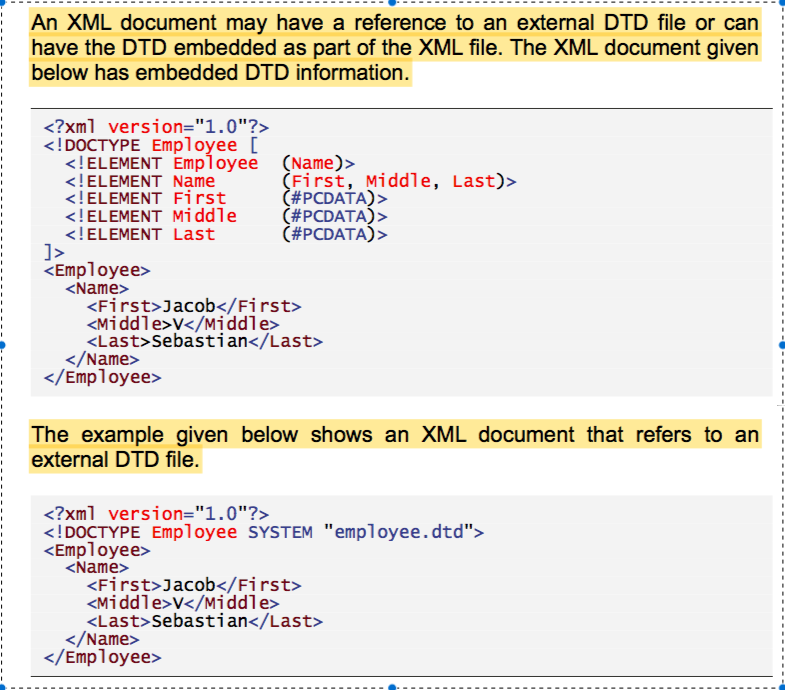
\includegraphics[width=.8\textwidth]{imgs/dtd.png}
    \end{block}
\end{frame}

\begin{frame}
    \frametitle{Elementi per la definizione degli schemi xml}
    \framesubtitle{Principi Document Type Definition}
    \addtocounter{nframe}{1}

    \begin{block}{Document Type Definition (DTD)}
        Una document type definition (DTD) descrive le regole relative alla struttura di un documento XML.
    \end{block}

    \begin{block}{Document Type Definition (DTD)}
        Una DTD dichiara gli elementi, gli attributi, le entità e le notazioni ammessi in un documento XML.
    \end{block}

\end{frame}


\begin{frame}
    \frametitle{Elementi per la definizione degli schemi xml}
    \framesubtitle{Principi Document Type Definition}
    \addtocounter{nframe}{1}

    \begin{block}{well-formed document != valid document}
         Se un documento XML manca di riferirsi ad una DTD oppure non rispetta le regole di una DTD, esso può essere tutt'al più ben formato, ma sicuramente non può essere valido.
    \end{block}
\end{frame}

\begin{frame}
    \frametitle{Elementi per la definizione degli schemi xml}
    \framesubtitle{Principi Document Type Definition}
    \addtocounter{nframe}{1}

    \begin{block}{Document Type Definition (DTD)}
        La validazione dei documenti XML è alla base della condivisione e scambio dati in quanto è possibile confidare sulla natura dei dati trasmessi.
    \end{block}
   \textit{Attenzione: non possiamo validare la correttezza della semantica dei dati!}
\end{frame}

\begin{frame}
    \frametitle{Elementi per la definizione degli schemi xml}
    \framesubtitle{Principi Document Type Definition}
    \addtocounter{nframe}{1}

    \begin{block}{Document Type Definition (DTD)}
         L'associazione tra documento XML e DTD viene realizzata tramite una dichiarazione inclusa nel prologo all'inizio del documento.
    \end{block}

    \begin{block}{Root element and content}
        La DTD dichiara l'elemento radice del vocabolario e il suo \textit{content model} (children elements).
    \end{block}
   
\end{frame}

\begin{frame}
    \frametitle{Elementi per la definizione degli schemi xml}
    \framesubtitle{Principi Document Type Definition}
    \addtocounter{nframe}{1}

    \begin{block}{Element Declaration (con figli)}
        \begin{center}\texttt{<!ELEMENT element-name (child-element1, child-element-2 ...)>}\end{center}
    \end{block}

    \begin{block}{Element Declaration (solo testo)}
    \begin{center}\texttt{<!ELEMENT element-name (\#PCDATA)>}\end{center}
    \end{block}
    \textit{Il Parsed Character Content designa contenuto testuale piano senza figli}
\end{frame}

\begin{frame}
    \frametitle{Elementi per la definizione degli schemi xml}
    \framesubtitle{Principi Document Type Definition}
    \addtocounter{nframe}{1}

    \begin{block}{Child Element Declaration}
        La dichiarazione di un elemento figlio, è analoga in tutto e per tutto alla dichiarazione dell'elemento radice. Cioè utilizzando l'etichetta \texttt{<!ELEMENT >}
    \end{block}

    \begin{block}{Element Declaration (root)}
     \textbf{La dichiarazione dell'elemento radice deve sempre essere la prima}
    \end{block}
\end{frame}

\begin{frame}
    \frametitle{Elementi per la definizione degli schemi xml}
    \framesubtitle{Principi Document Type Definition}
    \addtocounter{nframe}{1}

    \begin{block}{Modificatori}
        Nella dichiarazione di un elemento possono essere inclusi opzionalmente dei modificatori, per stabilire il numero di occorrenze degli elementi figli.
    \end{block}

    \begin{block}{Modificatori}
     + Una o più occorrenze\\ 
     ? Zero o una occorrenza\\
     * Zero o più occorrenze
    \end{block}
\end{frame}

\begin{frame}
    \frametitle{Elementi per la definizione degli schemi xml}
    \framesubtitle{Principi Document Type Definition}
    \addtocounter{nframe}{1}

    \begin{block}{Modificatori}
        \begin{center} \texttt{<!ELEMENT element-name (B, C)+ >} \end{center}
        \begin{center} \texttt{<!ELEMENT element-name (B+, C) >} \end{center}
        \begin{center} \texttt{<!ELEMENT element-name (B, C+) >} \end{center}
        \begin{center} \texttt{<!ELEMENT element-name (B+, C+) >} \end{center}
    \end{block}

     \textit{Se un elemento figlio deve presentarsi solo una volta, allora non c'è bisogno di modificatori}.
     \\\textit{Attenzione l'ordine dei figli nella dichiarazione è rilevante}
    
\end{frame}

\begin{frame}
    \frametitle{Elementi per la definizione degli schemi xml}
    \framesubtitle{Principi Document Type Definition}
    \addtocounter{nframe}{1}

    \begin{block}{Esercizio}
        \textit{Definire i seguenti elementi:}
        \begin{itemize}
            \item elemento root: TEI
            \item elementi figli:
            \begin{itemize}
                \item header (obbligatorio una occorrenza)
                \item facsimile (opzionale una occorrenza)
                \item text (obbligatorio almeno una occorrenza)
            \end{itemize}
        \end{itemize}
        \textit{header, facsimile, text hanno un content model testuale}
    \end{block}
\end{frame}


\begin{frame}
    \frametitle{Elementi per la definizione degli schemi xml}
    \framesubtitle{Principi Document Type Definition}
    \addtocounter{nframe}{1}

    \begin{block}{choice declaration}
    \begin{center} \texttt{<!ELEMENT element-name (child-a | child-b) >} \end{center}
    \end{block}

    \begin{block}{Dichiarazione di Choice}
        indicating a choice of just one, out of the list
    \end{block}

\end{frame}

\begin{frame}
    \frametitle{Elementi per la definizione degli schemi xml}
    \framesubtitle{Principi Document Type Definition}
    \addtocounter{nframe}{1}

    \begin{block}{Attributi}
    \begin{center} an attribute is declared with \texttt{<!ATTLIST >} element \end{center}
    \end{block}

    \begin{block}{Attributi}
        An attribute is the property of an element that describes the element’s content.
    \end{block}

\end{frame}

\begin{frame}
    \frametitle{Elementi per la definizione degli schemi xml}
    \framesubtitle{Principi Document Type Definition}
    \addtocounter{nframe}{1}

    \begin{block}{Attributi}
    \begin{center} \texttt{<!ATTLIST Element-name Attr-name Attr-type Attr-state? default-value?>} \end{center}
    \end{block}

    \begin{block}{Attributi}
        ``Element-name'' is the name of the element
        ``Attr-name'' is the attribute to be declared.
        ``Attr-type'' specifies the expected attribute’s data type
        The ``Attr-state'' denota una tra i tre stati possibili di un attributo 
        ``default-value'' if provided is the value to be used if the attribute is not supplied
    \end{block}

\end{frame}

\begin{frame}
    \frametitle{Elementi per la definizione degli schemi xml}
    \framesubtitle{TABELLA dei tipi}
    \addtocounter{nframe}{1}

    \begin{block}{Tipi di attributi}
    
    \end{block}
\end{frame}



\begin{frame}
    \frametitle{Elementi per la definizione degli schemi xml}
    \framesubtitle{}
    \addtocounter{nframe}{1}

    \begin{block}{Stato di attributi}
     The state can be any of \#IMPLIED (an optional attribute), \#REQUIRED (a compulsory attribute) or \#FIXED (a fixed value attribute that may not be changed) the value is provided as the default value. You cannot use the default-value with the \#REQUIRED state as you must supply a value for the attribute.
    \end{block}
\end{frame}

% slide con choice per gli attributi

\begin{frame}
    \frametitle{Elementi per la definizione degli schemi xml}
    \framesubtitle{}
    \addtocounter{nframe}{1}

    \begin{block}{Mixed content - DTD}
    \begin{center}\texttt{<!ELEMENT element-name (\#PCDATA|child-element)* >}\end{center}
    \end{block}

    \begin{block}{Mixed content XML}
    \begin{center}\texttt{<p>Ieri pomeriggio sono andato a <placeName>Pisa<placeName>, per un giro<p>}\end{center}
    \end{block}

\end{frame}


\begin{frame}
    \frametitle{Elementi per la definizione degli schemi xml}
    \framesubtitle{}
    \addtocounter{nframe}{1}

    \begin{block}{Esercizio}
        root: TEI
         figli: header(obbligatorio una volta sola) - facsimile(opzionale una volta sola) - testo(obbligatorio una o più volte)
         - testo è un mixed content con possibile elemento \texttt{<seg>} attributi: 
         - header: type:(fixed, CDATA ``intestazione''); lang(opzional, NMTOKEN)
         - facsimile: source:(obbligatorio)
         - testo: id(obbligatorio, contenuto id) type(opzionale contenuto testuale)
    \end{block}
\end{frame}


\begin{frame}
    \frametitle{Elementi per la definizione degli schemi xml}
    \framesubtitle{Principi Document Type Definition}
    \addtocounter{nframe}{1}

    \begin{block}{Empty elements}
    The only difference is that the child element name is substituted with the keyword “EMPTY”  
    \end{block}

    \begin{block}{Empy content}
    \begin{center}\texttt{<!ELEMENT element-name EMPTY>}\end{center}
    \end{block}


    \begin{block}{Empy content}
    \begin{center}\texttt{<lb />}\end{center}
    \end{block}

\end{frame}


\begin{frame}
    \frametitle{Elementi per la definizione degli schemi xml}
    \framesubtitle{Principi Document Type Definition}
    \addtocounter{nframe}{1}

    \begin{block}{Any elements}
 The content specification ``ANY'' when used in a declaration implies that any element as well as texts can be the child or content of the declared element.

    \end{block}

    \begin{block}{Any content}
    \begin{center}\texttt{<!ELEMENT element-name ANY >}\end{center}
    \end{block}
    
\end{frame}


\begin{frame}
    \frametitle{Elementi per la definizione degli schemi xml}
    \framesubtitle{Principi Document Type Definition}
    \addtocounter{nframe}{1}

    \begin{block}{Dichiarare il tipo del documento XML}
        The document type declaration is placed in the xml document prolog; between
         the xml declaration and the root element.

    \end{block}

    \begin{block}{Dichiarare il tipo del documento XML}
        re-usability reasons, and then link it to the xml document and any other xml document through its URL
    \end{block}

\end{frame}

\begin{frame}
    \frametitle{Elementi per la definizione degli schemi xml}
    \framesubtitle{Principi Document Type Definition}
    \addtocounter{nframe}{1}

    \begin{block}{DOCTYPE}
    \begin{center}\texttt{<!DOCTYPE root-element SYSTEM ``External DTD’s URL'' [Internal DTD ]>}\end{center}
    \begin{center}\texttt{<!DOCTYPE root-element [Internal DTD] >}\end{center}
    \begin{center}\texttt{<!DOCTYPE root-element SYSTEM ``Ext-DTD URL'' >}\end{center}
        
    \end{block}


\end{frame}

\begin{frame}
    \frametitle{Elementi per la definizione degli schemi xml}
    \framesubtitle{Principi Document Type Definition}
    \addtocounter{nframe}{1}

    \begin{block}{Esercizi}
    \begin{itemize}
        \item includere all'interno di un documento XML la dichiarazione del tipo, definire internamente gli elementi e gli attributi e validare.
        \item inserire nel prologo di un documento XML la dichiarazione del tipo di documento e validare.
    \end{itemize}
    \end{block}

    \textit{creare un file esterno con estensione .dtd prima di includerlo nel prologo XML.}

\end{frame}

\begin{frame}
    \frametitle{Elementi per la definizione degli schemi xml}
    \framesubtitle{Principi Document Type Definition}
    \addtocounter{nframe}{1}

    \begin{block}{Entity}
        Per includere dati da diverse fonti, DTD prevede l'uso di entità. Due tipologie di entità sono state definite: general entities e parameter entities.
    \end{block}

    \begin{block}{Entity: generiche e parametriche}
    \begin{itemize}
        \item le general entities vengono espanse nel documento XML
        \item le parameter entities vengono espanse nel documento DTD
    \end{itemize}
    \end{block}
    
\end{frame}

\begin{frame}
    \frametitle{Elementi per la definizione degli schemi xml}
    \framesubtitle{Principi Document Type Definition}
    \addtocounter{nframe}{1}

    \begin{block}{Entity}
    \begin{itemize}
        \item  Le general entities si possono classificare in interne ed esterne; che a loro volta possono essere parsed oppure unparsed.
        \item Le parameter entities si possono classificare in interne ed esterne; che  possono essere solo parsed.
    \end{itemize}
    \end{block}
    
\end{frame}

\begin{frame}
    \frametitle{Elementi per la definizione degli schemi xml}
    \framesubtitle{Principi Document Type Definition}
    \addtocounter{nframe}{1}

    \begin{block}{Entity}
     Internal general entities help include special characters in an xml document,
     that would otherwise make an xml document become malformed if included
     literally.
    \end{block}

\end{frame}

\begin{frame}
    \frametitle{Elementi per la definizione degli schemi xml}
    \framesubtitle{Principi Document Type Definition}
    \addtocounter{nframe}{1}

    \begin{block}{Internal General Entity: Sintassi}
    \begin{center}\texttt{<!ENTITY entity-name ``replacement-string'' or ``hexadecimal-code'' >}\end{center}
    \end{block}

\end{frame}

\begin{frame}
    \frametitle{Elementi per la definizione degli schemi xml}
    \framesubtitle{Principi Document Type Definition}
    \addtocounter{nframe}{1}

    \begin{block}{Internal General Entity: Sintassi}
        To use the entity name in the element content simply attach the ampersand to
        the beginning of the entity name and append the semi colon to the end like
        this; \&entity-name;
        \\ may include well formed xml elements.
    \end{block}

    \begin{block}{Internal General Entity: Sintassi}
    \begin{center}\texttt{<!ENTITY firma ``Angelo Mario Del Grosso''>}\end{center}
    \begin{center}\texttt{<p><salutation>\&firma;<salutation></p>}\end{center}
    \end{block}

\end{frame}

\begin{frame}
    \frametitle{Elementi per la definizione degli schemi xml}
    \framesubtitle{Principi Document Type Definition}
    \addtocounter{nframe}{1}

    \begin{block}{Internal General Entity: Esempio con UNICODE}
        Spesso le entità vengono utlizzate per dare un nome ai riferimenti a carattere.
    \end{block}

    \begin{block}{Internal General Entity: Sintassi}
    \begin{center}\texttt{<!ENTITY amaiuscola ``\&\#65;''>}\end{center}
    \begin{center}\texttt{<!ENTITY amaiuscola ``\&\#x0041;''>}\end{center}
    \begin{center}\texttt{<p><salutation>\&amaiuscola;ddio<salutation></p>}\end{center}
    \end{block}

\end{frame}

\begin{frame}
    \frametitle{Elementi per la definizione degli schemi xml}
    \framesubtitle{Principi Document Type Definition}
    \addtocounter{nframe}{1}

    \begin{block}{External General Entity}
        An xml document may be developed from other xml document located in different places. Grazie alle entità generiche esterne, questa eventualità diviene possibile.
    \end{block}

    \begin{block}{External General Entity: Sintassi}
    \begin{center}\texttt{<!ENTITY entity-name SYSTEM ``URL'' >}\end{center}
    \begin{center}\texttt{<!ENTITY salutation SYSTEM ``salut.xml.ent'' >}\end{center}
    \end{block}
    \textit{The URL points to the location of the external entity}
\end{frame}

\begin{frame}
    \frametitle{Elementi per la definizione degli schemi xml}
    \framesubtitle{Principi Document Type Definition}
    \addtocounter{nframe}{1}

    \begin{block}{External General Entity}
        External entities cannot contain a document type declaration as it will conflict with the main xml document type declaration. E' possibile utilizzare altre entità all'interno delle entità esterne. 
    \end{block}

    \begin{block}{General Entity}
     though declared in the DTD, must be used in the document and not in the DTD itself. 
    \end{block}
\end{frame}

\begin{frame}
    \frametitle{Elementi per la definizione degli schemi xml}
    \framesubtitle{Principi Document Type Definition}
    \addtocounter{nframe}{1}

    \begin{block}{Parameter Entity}
        Sono entità impiegabili all'interno del documento DTD. Ma non possono essere utilizzate all'interno del documento XML.
        \\ There are two types of parameter entity; the internal and the external parameter entities.
    \end{block}

    \begin{block}{Parameter Entity: Sintassi}
        \begin{center}\texttt{<!ENTITY \% entity-name ``replacement-string''>}\end{center}
        \begin{center}\texttt{<!ENTITY \% parameter-name SYSTEM ``URL'' >}\end{center}
    \end{block}
\end{frame}

\begin{frame}
    \frametitle{Elementi per la definizione degli schemi xml}
    \framesubtitle{Principi Document Type Definition}
    \addtocounter{nframe}{1}

    \begin{block}{Parameter Entity: Impiego}
    \begin{center}\texttt{<!ENTITY \% biblinfo ``(title,author?,cost?)''>}\end{center}
    \begin{center}\texttt{<!ELEMENT biblInfo \%biblinfo;>}\end{center}
    \end{block}

    \begin{block}{Parameter Entity: Impiego}
        \begin{center}\texttt{<!ENTITY \% biblInfo SYSTEM ``biblInfo.dtd'' >}\end{center}
        \begin{center}\texttt{<!ELEMENT listBibl (bib+) >}\end{center}
        \begin{center}\texttt{\%biblInfo;}\end{center}
    \end{block}
\end{frame}


\begin{frame}
    \frametitle{Elementi per la definizione degli schemi xml}
    \framesubtitle{Principi Document Type Definition}
    \addtocounter{nframe}{1}

    \begin{block}{Parameter Entity: utilità}
     When a parameter entity is inserted in the dtd, the parameter entity is replaced with the replacement content at execution time.
    \end{block}

    \begin{block}{Parameter Entity: utilità}
        This would make the dtd easier to develop and later maintained, if there are
        any changes to be made.
    \end{block}
\end{frame}

\begin{frame}
    \frametitle{Elementi per la definizione degli schemi xml}
    \framesubtitle{Principi Document Type Definition}
    \addtocounter{nframe}{1}

    \begin{block}{Parameter Entity: utilità}
        External parameter entities enable the modularization and linking of document
        type definitions.
    \end{block}

    \begin{block}{Parameter Entity: utilità}
        with external parameter entities you can embed modularized document type
        definitions from different locations to form a single and more complete
        document type definition.
    \end{block}
\end{frame}


% A parameter entity that is only a part of a complete declaration like above
% cannot appear in the internal definition subset of a dtd and must be placed in
% the external definition subset and referred to.

% Note that the parameter entity reference ”%Event-info;” was declared before it
% was used, and that “sport-calendar.dtd” was referred to in the external dtd
% subset as described in document 5.3 below:

% Internal parameter entities are declared in the dtd external subset

% Internal parameter entities are used much in the same way that the general
% entity references are used but they remain parts of the dtd and never appear
% in the document’s content. An internal parameter entity reference is
% represented as shown below: <!ENTITY % parameter-entity-name
% “replacement-content” >